\documentclass{article}
\usepackage{amsmath} % import of math elements
%\usepackage{mathtools} %import of other math elements
\usepackage{tikz} 
\usetikzlibrary{shapes,positioning,calc} 
\usetikzlibrary{positioning,matrix, arrows.meta}
\usetikzlibrary{decorations.pathreplacing}
\usepackage{listings}
\usepackage{color}
\usepackage{mathtools}
\DeclarePairedDelimiter\ceil{\lceil}{\rceil}
\DeclarePairedDelimiter\floor{\lfloor}{\rfloor}
\definecolor{dkgreen}{rgb}{0,0.6,0}
\definecolor{gray}{rgb}{0.5,0.5,0.5}
\definecolor{mauve}{rgb}{0.58,0,0.82}

\lstset{frame=tb,
  language=Bash,
  aboveskip=3mm,
  belowskip=3mm,
  showstringspaces=false,
  columns=flexible,
  basicstyle={\small\ttfamily},
  numbers=none,
  numberstyle=\tiny\color{gray},
  keywordstyle=\color{blue},
  commentstyle=\color{dkgreen},
  stringstyle=\color{mauve},
  breaklines=true,
  breakatwhitespace=true,
  tabsize=3
}

%-------------------------------------------------------
% Document information
%-------------------------------------------------------

\title{Algorithm and data structures} %Title 

\author{Roberto \textsc{Antoniello}} %author name

\begin{document}
\maketitle % show the title and author and date
%-------------------------------------------------------
%Introduction
%-------------------------------------------------------

\begin{center} In this file I will resume all the concepts I liked while studying the course of Algorithm and data structures.\end{center}

\section{Binary search}
This algorithm can be used only if you have a sorted array. Here how it works: \\
BinarySearch take a sorted array as input and return an index as output. So it returns the index of the found element or -1 if not found.\\
When it starts execution, the algorithm saves three variables \textbf{sx}, \textbf{dx} and \textbf{m}. The \textbf{m} variable is the index in the middle of the array, \textbf{sx} and \textbf{dx} are the first and the last index. It asks if the element is less or more than the element in \textbf{m} position. \\
Basically, if the element is x the question is: 
\textbf{x $<$ A[m]}  or  \textbf{x $>$ A[m]} ? 
We are reducing the search space by 2 every time because if it's less, our \textbf{dx} becomes \textbf{m}, otherwise our \textbf{sx} becomes \textbf{m+1}. \\
At the first iteration the search space is n elements, at the second it is $\cfrac{n}{2}$, at the third one it is $\cfrac{n}{2^2}$ and so on.\\
At the i° iteration it will be $\cfrac{n}{2^i}$.\\
During the last iteration the size of our array A is 1. So:\\
$\cfrac{n}{2^i} = 1 \Rightarrow n = 2^i \Rightarrow i = \log_2{n}$ \\
We have just said the amount of steps are $\log_2{n} \Rightarrow O(\log{n})$ \\
Here below there's an array as example with the initial value of sx,m and dx. \\

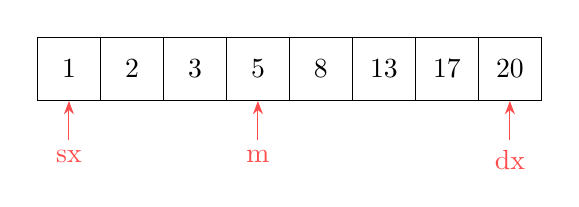
\begin{tikzpicture}
    \matrix (A) [matrix of nodes, nodes={draw, minimum size=8mm},
    column sep=-\pgflinewidth]{
        1 & 2 & 3 & 5 & 8 & 13 & 17 & 20\\
    };

    \foreach \i [evaluate=\i as \ni using {int(\i)},] in {1, 4, 8}{
        \pgfmathtruncatemacro{\half}{(\i + 1) / 2}
        \ifnum \i = 1
            \def\arrowlabel{sx}
        \else
            \ifnum \i = 4
                \def\arrowlabel{m}
            \else
                \def\arrowlabel{dx}
            \fi
        \fi
        \draw [{Stealth}-, red!70] (A-1-\ni.south) -- ++(-90:5mm) node[below] {\arrowlabel};
    }
\end{tikzpicture}

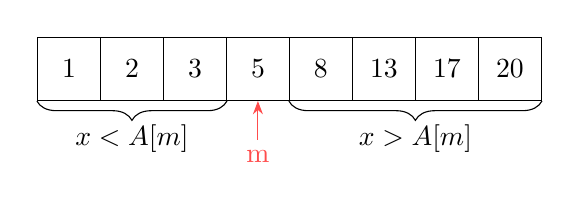
\begin{tikzpicture}
    \matrix (A) [matrix of nodes, nodes={draw, minimum size=8mm},
    column sep=-\pgflinewidth]{
        1 & 2 & 3 & 5 & 8 & 13 & 17 & 20\\
    };

    \foreach \i [evaluate=\i as \ni using {int(\i)},] in {4}{
        \pgfmathtruncatemacro{\half}{(\i + 1) / 2}
        \ifnum \i = 4
        		\def\arrowlabel{m}
        	\fi
        \draw [{Stealth}-, red!70] (A-1-\ni.south) -- ++(-90:5mm) node[below] {\arrowlabel};
    }

    % Brace for x < A[m]
    \draw [decorate,decoration={brace,amplitude=7pt,mirror},xshift=-1pt,yshift=-2pt]
        (A-1-1.south west) -- (A-1-3.south east) node[midway,below=5pt] {${x < A[m]}$};

    % Brace for x > A[m]
    \draw [decorate,decoration={brace,amplitude=7pt,mirror},xshift=-1pt,yshift=-2pt]
        (A-1-5.south west) -- (A-1-8.south east) node[midway,below=5pt] {${x > A[m]}$};
\end{tikzpicture}


I let you read the pseudocode here below. \\ \\ \\

\begin{lstlisting}[caption={\\\textit{Iterative version of the binary search algorithm.}}]
Algorithm BinarySearch(Array A[0,..,n-1]) --> index
	sx <-- 0
	dx <-- n
	index <-- -1
	while sx < dx do
		m <-- (sx+dx) / 2
		if x < A[m] then
			dx <-- m
		else if x = A[m] then
			index <-- m
		else
			sx <-- m+1
\end{lstlisting}

\section{Selection Sort}
So we know that to do a biinary search, we need a sorted array. \\
There are many solutions to sort an array with more or less complexity in time and space. \\
The first algorithm we're gonna see is the selection sort. This sorting algorithm is really simple, essentially it slides the array and when it find the minimum value it put it at the beginning in the right place. After this step we consider that element sorted and so on until we have the entire array sorted. \\
Let's see here below the pseudocode and then a quick and easy complexity analysis. \\

\begin{lstlisting}[caption={\\\textit{Selection sort algorithm.}}]
Algorithm SelectionSort(Array A[0,..,n-1]) 
	for k <-- 1 to n-2 do
		//finding the index m of minimum value between k and n-1
		m <-- k
		for j <-- k+1 to n-1 do
			if A[j] < A[m] then
				m <-- j
		swap A[m] with A[k]
\end{lstlisting}
The first for cycle ends at \textbf{n-2} because the last element is already sorted if we remember how it works the algorithm. \\
The second for cycle finds the minimum value starting from m position.\\
So, how many comparisons have I to do?\\
If we look at our array A, we can consider that at the k iteration we have \textbf{k} sorted elements on the left and \textbf{n-k-1} to sort on the right.\\

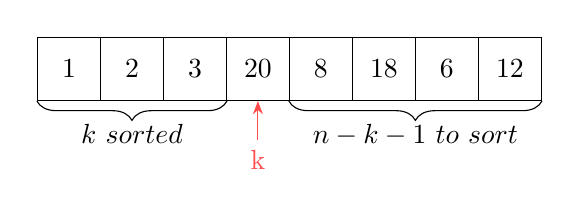
\begin{tikzpicture}
    \matrix (A) [matrix of nodes, nodes={draw, minimum size=8mm},
    column sep=-\pgflinewidth]{
        1 & 2 & 3 & 20 & 8 & 18 & 6 & 12\\
    };

    \foreach \i [evaluate=\i as \ni using {int(\i)},] in {4}{
        \pgfmathtruncatemacro{\half}{(\i + 1) / 2}
        \ifnum \i = 4
        		\def\arrowlabel{k}
        	\fi
        \draw [{Stealth}-, red!70] (A-1-\ni.south) -- ++(-90:5mm) node[below] {\arrowlabel};
    }

    % Brace for x < A[m]
    \draw [decorate,decoration={brace,amplitude=7pt,mirror},xshift=-1pt,yshift=-2pt]
        (A-1-1.south west) -- (A-1-3.south east) node[midway,below=5pt] {${k \ sorted}$};

    % Brace for x > A[m]
    \draw [decorate,decoration={brace,amplitude=7pt,mirror},xshift=-1pt,yshift=-2pt]
        (A-1-5.south west) -- (A-1-8.south east) node[midway,below=5pt] {${n-k-1 \ to \ sort}$};
\end{tikzpicture}
 
 Basically we are doing this sum: \\
 $$\sum_{k=0}^{n-2}(n-k-1)$$
This is equal to sum every $n \in \mathcal{N}$ from 0 to n-2, so:\\
$$\sum_{k=0}^{n-2}(n-k-1) = \sum_{i=1}^{n+1} i = \cfrac{n \cdot (n-1)}{2}$$
This is the total of comparisons I have to do in this algorithm.
The complexity is thus $\Theta(n^2)$. \\
We can say also that this amount of comparisons is always done because we do not set any condition to do these comparisons.

\section{Bubble sort}
The second sorting algorithm we're gonna see is Bubble sort.\\
This works by sliding the array and compare the current element with the previous one. The bigger element is moved in the next position. This make the bigger element go forward until there's another bigger than it. It's called bubble because these big values go forward like the bubbles in the water.\\
Let's do a simulation here below.\\

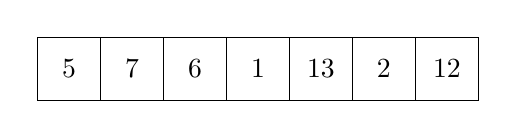
\begin{tikzpicture}
    \matrix (A) [matrix of nodes, nodes={draw, minimum size=8mm},
    column sep=-\pgflinewidth]{
        5 & 7 & 6 & 1 & 13 & 2 & 12\\
    };
\end{tikzpicture}

let's do the first iteration.\\

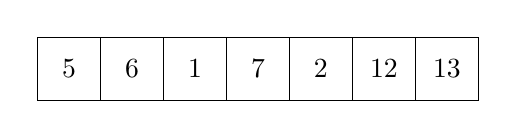
\begin{tikzpicture}
    \matrix (A) [matrix of nodes, nodes={draw, minimum size=8mm},
    column sep=-\pgflinewidth]{
        5 & 6 & 1 & 7 & 2 & 12 & 13\\
    };
\end{tikzpicture}


\begin{center}We compared 5 with 7 $\Rightarrow$ already sorted. \\
Then 7 with 6 $\Rightarrow$ swap. \\
Then 7 with 1 $\Rightarrow$ swap. \\
Then 7 with 13 $\Rightarrow$ already sorted. \\
Then 13 with 2 $\Rightarrow$ swap. \\
Then 13 with 12 $\Rightarrow$ swap. \\

In the next iteration I'll slide again until the entire array is sorted.\\ \end{center}

Now we consider the pseudocode.\\

\begin{lstlisting}[caption={\\\textit{Bubble sort algorithm.}}]
Algorithm BubbleSort(Array A[0,..,n-1]) 
	i <-- 1
	do
		swapped <-- false
		for j <--1 to n-i do
			if A[j] < A[j-1] then
				swap A[j] with A[j-1]
				swapped <-- true
		i <-- i + 1
	while swapped and i < n	
\end{lstlisting}

The for cycle ends at \textbf{n-i} because the last \textbf{i} elements are already sorted as we discussed how it work bubble sort. The external do while cycle ends when we did an iteration without any swap of elements or we reached the \textbf{n-1} iteration. The \textbf{i $<$ n} condition saves us the last iteration without any swap sliding the already sorted array.\\
Let's analyse the comparisons. Inside the main for cycle we do \textbf{n-i} comparisons where \textbf{i} starts at \textbf{1} to \textbf{n-1}. We're doing this sum:\\
$$\sum_{i=1}^{n-1}(n-i) = \sum_{k=1}^{n-1}k = \cfrac{n \cdot (n+1)}{2} = \Theta(n^2)$$
Again, the total amount of comparisons is in the order of $n^2$, but there's a difference between selection sort and bubble sort. That's because here we have this amount of comparisons only in the worst case(reverse sorted array), but in the best case(array already sorted) we can easily see that the amount of comparisons is in the order of $\Theta(n)$ because we just slide one time the array and then the algorithm ends doing \textbf{n-1} comparisons.

\section{Merge sort}
Let's consider the idea of having two already sorted arrays.\\
How can we build an array that contains all the elements sorted?\\
The first option we can think is to do a bubble sort and surely we can do it in $n^2$ steps. \\
Anyway there's a clever way to do this and it's called \textbf{merge}.

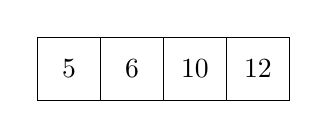
\begin{tikzpicture}
    \matrix (A) [matrix of nodes, nodes={draw, minimum size=8mm},
    column sep=-\pgflinewidth]{
        5 & 6 & 10 & 12 \\
    };
\end{tikzpicture}
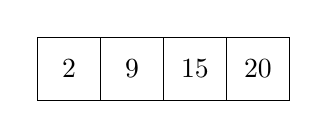
\begin{tikzpicture}
    \matrix (A) [matrix of nodes, nodes={draw, minimum size=8mm},
    column sep=-\pgflinewidth]{
         2 & 9 & 15 & 20\\
    };
\end{tikzpicture}

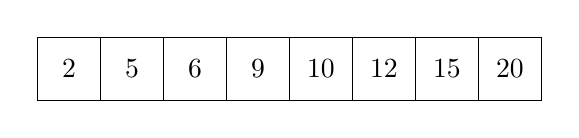
\begin{tikzpicture}
    \matrix (A) [matrix of nodes, nodes={draw, minimum size=8mm},
    column sep=-\pgflinewidth]{
         2 & 5 & 6 & 9 & 10 & 12 & 15 & 20\\
    };
\end{tikzpicture}
\subsection{merge}
The merge procedure works as this: \\
at every step I compare the first two numbers and the mininum go in the final array. When one of the sorted array ends, I append the remaining numbers of the other array without compare anything.\\
How much it costs? Well, every compare will put an element in the right place, so in the worst case I compare all the elements and the remaining is only one element in the other array. So the merge procedure has complexity in the order of $O(n)$ because I do \textbf{n-1} comparisons in the worst case.\\
Here below I drop the pseudocode of a simple version of the merge procedure, which it isn't perfectly optimized in memory.\\

\begin{lstlisting}[caption={\\\textit{Merge algorithm.}}]
Algorithm Merge(Array B[0,..,lb-1], Array C[0,..,lc-1]) --> Array 
	Be X[o,..,lb+lc-1] an array
	i1,i2,k <-- 0
	while i1 < lb and i2 < lc do
		if B[i1] <= C[i2] then
			X[k] <-- B[i1]
			i1 <-- i1+1
		else
			X[k] <-- C[i2]
			i2 <-- i2+1
		k <-- k +1
	//The remaining elements are in B	
	if i1 < lb then
		for j <- i1 to lb-1 do
			X[k] <-- B[j]
			k <-- k+1
	else
		//The remaining elements are in C
		for j <--i2 to lc-1 do
			X[k] <-- C[j]
			k <-- k+1
	return x
\end{lstlisting}
\leavevmode \\ \\ \\ \\ \\ \\ \\ \\ \\ \\ \\
Let's remember two corollaries we will use later:\\
$$\sum_{i = 0}^{k-1} 2^i = 2^k -1$$
If you convert in binary, you can see that all the power of two are 1 with all zeros behind. If you sum those all you obtain $2^k$. \\
Now the second corollary:\\
$\forall n \in \mathcal{N} \ \exists $ a power of two $N \ : \ n \leq N \leq 2n$

\subsection{Using merge inside Merge sort}
Let's define Merge sort recursively:\\
If $n \leq 1$ then A is already sorted, I do nothing.\\
Otherwise:\\
\begin{enumerate}
\item Divide A by two equal parts.
\item Sort them separately.
\item Merge them in a unique array(merge algorithm)
\end{enumerate}

I'll show here below the pseudocode of the Merge sort, which use our merge algorithm written before. So this algorithm suffers too of the missing optimization in memory, but it will be good enough to do our complexity analysis.

\begin{lstlisting}[caption={\\\textit{Merge algorithm.}}]
Algorithm Mergesort(Array A[0,..,n-1)
	If n > 1 then
		m <-- n / 2
		B <-- A[o,..,m-1]
		C <-- A[m,..,n-1]
		Mergesort(B)
		Mergesort(C)
	A <-- merge(B,C)
\end{lstlisting}
\leavevmode \\ \\ \\ \\ \\

\subsection{Amount of comparisons}

The amount of comparisons made are:\\
\begin{enumerate}
\item Comparisons of Mergesort(B).
\item Comparisons of Mergesort(C).
\item Comparisons of merge(B,C).
\end{enumerate}

The equation resulting from this observation is here below and we're going to solve it.

\begin{equation*}
	\left\{ \begin{aligned}
	0 \ \ \ \ \ \ \ \ \ \ \ \ \ \ \ \ \ \ \ \ \ \ \ \ \ \ \ \ \ \ \ \ \ \ \ \ \ \ \ \ \ \ \ \ \ \ \ \ if \ n \leq 1 \\
	C\left(\floor*{\cfrac{n}{2}}\right) + 	C\left(\ceil*{\cfrac{n}{2}}\right) + C_{merge}(n) \ \ otherwise
	\end{aligned} \right.
\end{equation*}
\leavevmode \\ \\
Let's consider our \textbf{n} is even. The equation becomes:\\

\begin{equation*}
	\left\{ \begin{aligned}
	0 \ \ \ \ \ \ \ \ \ \ \ \ \ \ \ \ \ \ \ \ \ \ \ \ \ \ \ \ \ \ \ \ \ \ \ \ if \ n \leq 1 \\
	2C\left(\cfrac{n}{2}\right) + C_{merge}(n) \ \ otherwise
	\end{aligned} \right.
\end{equation*}

By solving this equation we're going to demonstrate the amount of comparisons Mergesort do until we have a sorted array in the end. We'll solve by substitution.\\
\begin{large}

$C(n) = 2C\left(\cfrac{n}{2}\right) + n-1 =$

$2\left[2C\left(\cfrac{n}{2^2}\right) + \cfrac{n}{2} -1 \right] + n-1=$

$2^2\cdot C\left(\cfrac{n}{2^2}\right) + n-2 + n-1=$

$2^2\cdot \left[2C\left(\cfrac{n}{2^3}\right) + \cfrac{n}{2^2} -1 \right] + n-2 n-1=$

$2^3C\left(\cfrac{n}{2^3}\right) + n-2^3 + n-2^1 + n - 2^0=$

$$2^3C\left(\cfrac{n}{2^3}\right) + 3n - \sum_{i=0}^{3-1}2^i=$$

$$2^kC\left(\cfrac{n}{2^k}\right) + kn - \sum_{i=0}^{k-1}2^i=$$

We know that $\sum_{i=0}^{k-1}2^i = 2^k  -1$ \\
Now let's manipulate to the base case:\\
$\cfrac{n}{2^k} = 1 \Rightarrow n = 2^k \Rightarrow k = \log_2(n)$
Let's substitute now:\\
$C(n) = n\cdot C(1) + n\cdot\log_2{n} - n + 1 $ \\

We know that $C(1) = 0$, so the amount of comparisons is in the order of $$\Theta(n\cdot\log(n))$$
\end{large}
What about the recursion stack of memory?\\
If we still consider n as even, then the equation is:\\
$$H(n) = 1 + H\left(\cfrac{n}{2}\right)$$
If we do similar manipulation as made a moment ago we can reach this result:\\
$$H(n) = \Theta(\log(n))$$

\section{Quick sort}
The recursive definition of Quick sort is pretty similar to the Merge sort one. This is because both algorithm are using the Divide et impera technique.\\
The difference between these two sortin algorithm is quite simple. Inside Mergesort the complex part was the final merge, instead here we're going to see that the complex part will be the first one of dividing the problem in more problem of minor size.
\begin{center}
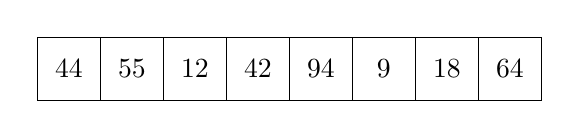
\begin{tikzpicture}
    \matrix (A) [matrix of nodes, nodes={draw, minimum size=8mm},
    column sep=-\pgflinewidth]{
         44 & 55 & 12 & 42 & 94 & 9 & 18 & 64\\
    };
\end{tikzpicture}

We choose a pivot element, 42 for example. if $ n \leq pivot$  then those elements go on the left of pivot, otherwise they go on the right.\\
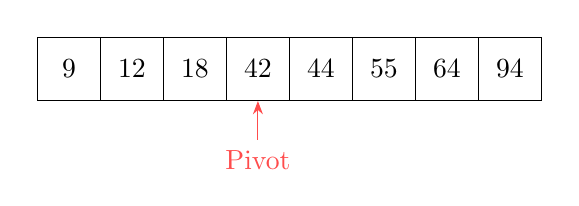
\begin{tikzpicture}
    \matrix (A) [matrix of nodes, nodes={draw, minimum size=8mm},
    column sep=-\pgflinewidth]{
         9 & 12 & 18 & 42 & 44 & 55 & 64 & 94\\
    };
    \foreach \i [evaluate=\i as \ni using {int(\i)},] in {4}{
        \pgfmathtruncatemacro{\half}{(\i + 1) / 2}
        \ifnum \i = 4
        		\def\arrowlabel{Pivot}
        	\fi
        \draw [{Stealth}-, red!70] (A-1-\ni.south) -- ++(-90:5mm) node[below] {\arrowlabel};
    }
\end{tikzpicture}
\end{center}

How to do this? We use an algorithm we will call partition. We define two index \textbf{sx} and \textbf{dx}. sx starts at the beginning of array while dx starts from the end.\\
\begin{enumerate}
\item dx starts sliding until it finds an element $\leq$ of pivot.
\item sx then starts sliding until it finfd an element $>$ of pivot.
\item Then swap sx with dx.
\item If sx $<$ dx, then swap dx with the pivot.
\end{enumerate}

Let's give a look to the pseudocode of partition here below.\\

\begin{lstlisting}[caption={\\\textit{Partition algorithm.}}]
Algorithm Partition(Array A[0,..,n-1],index i,index f) --> index
	pivot <-- A[i]
	sx <-- i
	dx <-- f
	while sx < dx do
		do
			dx <-- dx-1
		while A[dx] > pivot
		do
			sx <-- sx+1
		while sx < dx and A[sx] <= pivot
		if sx < dx then
			swap A[sx] with A[dx]
	swap A[i] with A[dx]
	return dx
\end{lstlisting}

The amount of comparisons is in the order of $O(n)$.\\
Now let's see the pseudocode of Quicksort that use partition.\\

\begin{lstlisting}[caption={\\\textit{Quicksort algorithm.}}]
Algorithm Quicksort(Array A[0,..,n-1])
	Quicksort(A,0,n)
\end{lstlisting}

\begin{lstlisting}[caption={\\\textit{Quicksort procedure.}}]
Procedure Quicksort(Array A[0,..,n-1],index i,index f)
	if f - i > 1 then
		m <-- partition(A,i,f)
		Quicksort(A,i,m)
		Quicksort(A,m+1,f)
\end{lstlisting}

We have now to calculate the amount of comparisons we do in this algorithm. To do this let's consider this aspect:\\

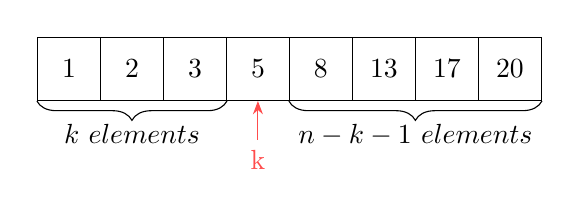
\begin{tikzpicture}
    \matrix (A) [matrix of nodes, nodes={draw, minimum size=8mm},
    column sep=-\pgflinewidth]{
        1 & 2 & 3 & 5 & 8 & 13 & 17 & 20\\
    };

    \foreach \i [evaluate=\i as \ni using {int(\i)},] in {4}{
        \pgfmathtruncatemacro{\half}{(\i + 1) / 2}
        \ifnum \i = 4
        		\def\arrowlabel{k}
        	\fi
        \draw [{Stealth}-, red!70] (A-1-\ni.south) -- ++(-90:5mm) node[below] {\arrowlabel};
    }

    % Brace for x < A[m]
    \draw [decorate,decoration={brace,amplitude=7pt,mirror},xshift=-1pt,yshift=-2pt]
        (A-1-1.south west) -- (A-1-3.south east) node[midway,below=5pt] {${k \ elements}$};

    % Brace for x > A[m]
    \draw [decorate,decoration={brace,amplitude=7pt,mirror},xshift=-1pt,yshift=-2pt]
        (A-1-5.south west) -- (A-1-8.south east) node[midway,below=5pt] {${n - k - 1 \ elements}$};
\end{tikzpicture}

Basically, we have $C(k)$ on the left and $C(n-k-1)$ on the right.\\
We know also that $C_{part}(n) = n$

So the total amount of comparisons is made of $n + C(k) + C(n-k-1)$

\subsection{Worst case}
It's easily to see that the worst case happen when $k=0$ or $k=n-1$.
\begin{large}
\begin{equation*}
	\left\{ \begin{aligned}
	0 \ \ \ \ \ \ \ \ \ \ \ \ \ \ \ \ \ \ \ \ \ \ \ \ \ \ \ \ \ \ \ \ \ \ \ \ \ \ \ \ \ \ \ \ \  \ \ \ \ \ \ \ \ \ \ \ \ \ \ \ \ \ \ \ \ \ \ \ \ if \ n \leq 1 \\
	n + max \left(C_w(k) + C_w(n-k-1) : k =0,..,n-1 \right) \ \ otherwise
	\end{aligned} \right.
\end{equation*}

$C_w(n) = n + C_w(n-1) = n + n-1 + C_w(n-2) = $

$ n + n-1 + n-2 + C_w(n-3)=\ldots = $
$$n + n-1 + n-2 + \ldots + 2 + C(1) = \sum_{i=1}^n i = \cfrac{n \cdot (n+1)}{2}  \Rightarrow \Theta(n^2)$$
\end{large}
Well well well, we have built this complex algorithm but in the worst case we just found that the amount of comparisons is in the order of $n^2$ such as a Selection sort or a Bubble sort. \\
There's something to say about this anyway, because this case is very rare and you have to find it manually to make it happens for real.\\

\subsection{Best case}
The best case happens when the partition is balanced. We just obtain similar result as we did for Mergesort.
\begin{large}
\begin{equation*}
	\left\{ \begin{aligned}
	0 \ \ \ \ \ \ \ \ \ \ \ \ \ \ \ \ \ \ \ \ \ \ \ \ \ \ \ \ \ \ \ \ \ \ \ \ \ \ \ \ \ \ \ \ \  \ \ \ \ \ \ \ \ \ \ \ \ \ \ \ \ \ \ \ \ \ \ \ \ if \ n \leq 1 \\
	n + min \left(C_w(k) + C_w(n-k-1) : k =0,..,n-1 \right) \ \ otherwise
	\end{aligned} \right.
\end{equation*}

$C_b(n) \simeq n + 2C_b\left(\cfrac{n}{2}\right) \Rightarrow$
$C_b(n) \simeq n\cdot \log_2(n)$
\end{large}

\subsection{Average case}
The average case is a little bit more difficult to analyze, but don't worry we'll make it too.\\
\begin{large}
\begin{equation*}
	\left\{ \begin{aligned}
	0 \ \ \ \ \ \ \ \ \ \ \ \ \ \ \ \ \ \ \ \ \ \ \ \ \ \ \ \ \ \ \ \ \ \ \ \ \ \ \ \ \ \ \ \ \  \ \ \ \ \ \ \ \ \ \ \ \ \ \ \ \ \ \ \ \ \ \ \ \ if \ n \leq 1 \\
	\cfrac{\sum_{k=0}^{n-1} C_n + C(k) + C(n-k-1)}{n} \ \ \ \ \ \ \ \ \ \ \ \ \ \ \ \ \ \  \ \ \ \ \ \ otherwise
	\end{aligned} \right.
\end{equation*}

Let's manipulate this bad fraction.\\
$$C(n) = \cfrac{1}{n}\sum_{k=0}^{n-1} n + \cfrac{1}{n}\sum_{k=0}^{n-1}C(k) + \cfrac{1}{n}\sum_{k=0}^{n-1}C(n-k-1)$$
The first summation is equal to $n$.\\
The second and the third are symmetrical because the second sum from 0 to n-1 and the third do the reverse thing. So:\\
$$C(n) = n + \cfrac{2}{n} \sum_{i=0}^{n-1}C(i) = n + \cfrac{2}{n} \sum_{i=2}^{n-1}C(i)$$
$C(0)=C(1)=0 \Rightarrow$ we can start from $i=2$
Let's update the equation after these steps.\\
\begin{equation*}
	\left\{ \begin{aligned}
	0 \ \ \ \ \ \ \ \ \ \ \ \ \ \ \ \ \ \ \ \ \ \ \ \ \ \ \ \ \ \ \ \ \ \ \ \ \ \ \ \ \ \ \ \ if \ n \leq 1 \\
	n + \cfrac{2}{n} \sum_{i=2}^{n-1} C(i) \ \ \ \ \ \ \ \ \ \ \ \ \ \ \ \ \ \  \ \ \ \ \ \ \ \ otherwise
	\end{aligned} \right.
\end{equation*}
Now we'll demonstrate by induction that $C(n) \leq 2n\cdot ln(n) \ by \ n \geq 1$
Base step: $n=1 \Rightarrow C(1) = 0 \Rightarrow 2ln(1) = 0 \Rightarrow OK$
Induction step: $$C(n) = n + \cfrac{2}{n} \sum_{i=2}^{n-1} C(i) \leq n + \cfrac{2}{n} \sum_{i=2}^{n-1} 2i\cdot ln(i) = n + \cfrac{4}{n} \sum_{i=2}^{n-1} i \cdot ln(i)$$

We'll make use of an integral to get the correct value of this summation and refactor this disequation.\\
$$\sum_{i=1}^{n-1} i \cdot ln(i) \leq \int_{2}^{n} x\cdot ln(x) dx$$
We can solve this integral by parts.\\
$$\int_{2}^{n} x\cdot ln(x) dx = \cfrac{x^2}{2} \cdot ln(x) - \int_{2}^{n} \cfrac{1}{x} \cdot \cfrac{x^2}{2} dx = \cfrac{x^2}{2} \cdot ln(x) - \cfrac{x^2}{4}$$
$\Rightarrow \left[\cfrac{x^2}{2} \cdot ln(x) - \cfrac{x^2}{4}\right]_2^n = \cfrac{n^2}{2}\cdot ln(n) - \cfrac{n^2}{4} - 2ln(2) + 1$

$2ln(2) + 1 \simeq 0$

So:\\
$$\sum_{i=1}^{n-1} i \cdot ln(i) \leq \cfrac{n^2}{2}\cdot ln(n) - \cfrac{n^2}{4}$$
Then we return to the original disequation and we update it:\\
$$ n + \cfrac{4}{n} \sum_{i=2}^{n-1} i \cdot ln(i) \leq n + \cfrac{4}{n} \cdot \left(\cfrac{n^2}{2}\cdot ln(n) - \cfrac{n^2}{4} \right)$$
$= n + 2n\cdot ln(n) -n = 2n\cdot ln(n) \Rightarrow Demonstrated.$

So we have demonstrated that in average case: \\ 
$C(n) \leq 2n\cdot ln(n) \simeq 1.39n\cdot ln(n)$\\

Regarding the use of the stack for recursion, we can say that such as merge sort this version is less optimized about memory because we have two recursions call in queue.\\
In average and best case we have a complexity in space in the order of $\Theta(log(n))$ but when the array is already sorted or almost sorted the amount of stack memory is in the order of $\Theta(n)$.
\end{large}
\section{Binary Trees}

\end{document}
